% Created by tikzDevice version 0.11 on 2018-04-21 16:54:48
% !TEX encoding = UTF-8 Unicode
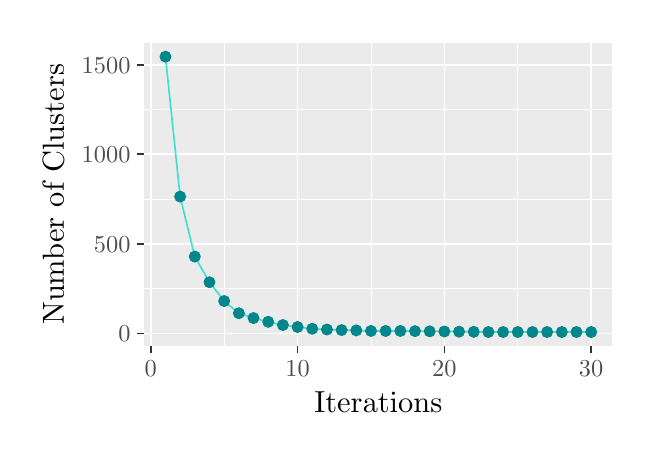
\begin{tikzpicture}[x=1pt,y=1pt]
\definecolor{fillColor}{RGB}{255,255,255}
\path[use as bounding box,fill=fillColor,fill opacity=0.00] (0,0) rectangle (216.81,144.54);
\begin{scope}
\path[clip] (  0.00,  0.00) rectangle (216.81,144.54);
\definecolor{drawColor}{RGB}{255,255,255}
\definecolor{fillColor}{RGB}{255,255,255}

\path[draw=drawColor,line width= 0.6pt,line join=round,line cap=round,fill=fillColor] (  0.00,  0.00) rectangle (216.81,144.54);
\end{scope}
\begin{scope}
\path[clip] ( 42.09, 29.59) rectangle (211.31,139.04);
\definecolor{fillColor}{gray}{0.92}

\path[fill=fillColor] ( 42.09, 29.59) rectangle (211.31,139.04);
\definecolor{drawColor}{RGB}{255,255,255}

\path[draw=drawColor,line width= 0.3pt,line join=round] ( 42.09, 50.23) --
	(211.31, 50.23);

\path[draw=drawColor,line width= 0.3pt,line join=round] ( 42.09, 82.60) --
	(211.31, 82.60);

\path[draw=drawColor,line width= 0.3pt,line join=round] ( 42.09,114.97) --
	(211.31,114.97);

\path[draw=drawColor,line width= 0.3pt,line join=round] ( 71.00, 29.59) --
	( 71.00,139.04);

\path[draw=drawColor,line width= 0.3pt,line join=round] (124.05, 29.59) --
	(124.05,139.04);

\path[draw=drawColor,line width= 0.3pt,line join=round] (177.10, 29.59) --
	(177.10,139.04);

\path[draw=drawColor,line width= 0.6pt,line join=round] ( 42.09, 34.04) --
	(211.31, 34.04);

\path[draw=drawColor,line width= 0.6pt,line join=round] ( 42.09, 66.41) --
	(211.31, 66.41);

\path[draw=drawColor,line width= 0.6pt,line join=round] ( 42.09, 98.78) --
	(211.31, 98.78);

\path[draw=drawColor,line width= 0.6pt,line join=round] ( 42.09,131.15) --
	(211.31,131.15);

\path[draw=drawColor,line width= 0.6pt,line join=round] ( 44.48, 29.59) --
	( 44.48,139.04);

\path[draw=drawColor,line width= 0.6pt,line join=round] ( 97.53, 29.59) --
	( 97.53,139.04);

\path[draw=drawColor,line width= 0.6pt,line join=round] (150.57, 29.59) --
	(150.57,139.04);

\path[draw=drawColor,line width= 0.6pt,line join=round] (203.62, 29.59) --
	(203.62,139.04);
\definecolor{drawColor}{RGB}{64,224,208}

\path[draw=drawColor,line width= 0.6pt,line join=round] ( 49.79,134.06) --
	( 55.09, 83.50) --
	( 60.39, 61.82) --
	( 65.70, 52.56) --
	( 71.00, 45.76) --
	( 76.31, 41.36) --
	( 81.61, 39.61) --
	( 86.92, 38.25) --
	( 92.22, 37.09) --
	( 97.53, 36.37) --
	(102.83, 35.73) --
	(108.14, 35.47) --
	(113.44, 35.27) --
	(118.74, 35.14) --
	(124.05, 34.95) --
	(129.35, 34.95) --
	(134.66, 34.95) --
	(139.96, 34.89) --
	(145.27, 34.82) --
	(150.57, 34.76) --
	(155.88, 34.69) --
	(161.18, 34.63) --
	(166.49, 34.56) --
	(171.79, 34.56) --
	(177.10, 34.56) --
	(182.40, 34.56) --
	(187.70, 34.56) --
	(193.01, 34.56) --
	(198.31, 34.56) --
	(203.62, 34.56);
\definecolor{drawColor}{RGB}{0,134,139}
\definecolor{fillColor}{RGB}{0,134,139}

\path[draw=drawColor,line width= 0.4pt,line join=round,line cap=round,fill=fillColor] ( 49.79,134.06) circle (  1.96);

\path[draw=drawColor,line width= 0.4pt,line join=round,line cap=round,fill=fillColor] ( 55.09, 83.50) circle (  1.96);

\path[draw=drawColor,line width= 0.4pt,line join=round,line cap=round,fill=fillColor] ( 60.39, 61.82) circle (  1.96);

\path[draw=drawColor,line width= 0.4pt,line join=round,line cap=round,fill=fillColor] ( 65.70, 52.56) circle (  1.96);

\path[draw=drawColor,line width= 0.4pt,line join=round,line cap=round,fill=fillColor] ( 71.00, 45.76) circle (  1.96);

\path[draw=drawColor,line width= 0.4pt,line join=round,line cap=round,fill=fillColor] ( 76.31, 41.36) circle (  1.96);

\path[draw=drawColor,line width= 0.4pt,line join=round,line cap=round,fill=fillColor] ( 81.61, 39.61) circle (  1.96);

\path[draw=drawColor,line width= 0.4pt,line join=round,line cap=round,fill=fillColor] ( 86.92, 38.25) circle (  1.96);

\path[draw=drawColor,line width= 0.4pt,line join=round,line cap=round,fill=fillColor] ( 92.22, 37.09) circle (  1.96);

\path[draw=drawColor,line width= 0.4pt,line join=round,line cap=round,fill=fillColor] ( 97.53, 36.37) circle (  1.96);

\path[draw=drawColor,line width= 0.4pt,line join=round,line cap=round,fill=fillColor] (102.83, 35.73) circle (  1.96);

\path[draw=drawColor,line width= 0.4pt,line join=round,line cap=round,fill=fillColor] (108.14, 35.47) circle (  1.96);

\path[draw=drawColor,line width= 0.4pt,line join=round,line cap=round,fill=fillColor] (113.44, 35.27) circle (  1.96);

\path[draw=drawColor,line width= 0.4pt,line join=round,line cap=round,fill=fillColor] (118.74, 35.14) circle (  1.96);

\path[draw=drawColor,line width= 0.4pt,line join=round,line cap=round,fill=fillColor] (124.05, 34.95) circle (  1.96);

\path[draw=drawColor,line width= 0.4pt,line join=round,line cap=round,fill=fillColor] (129.35, 34.95) circle (  1.96);

\path[draw=drawColor,line width= 0.4pt,line join=round,line cap=round,fill=fillColor] (134.66, 34.95) circle (  1.96);

\path[draw=drawColor,line width= 0.4pt,line join=round,line cap=round,fill=fillColor] (139.96, 34.89) circle (  1.96);

\path[draw=drawColor,line width= 0.4pt,line join=round,line cap=round,fill=fillColor] (145.27, 34.82) circle (  1.96);

\path[draw=drawColor,line width= 0.4pt,line join=round,line cap=round,fill=fillColor] (150.57, 34.76) circle (  1.96);

\path[draw=drawColor,line width= 0.4pt,line join=round,line cap=round,fill=fillColor] (155.88, 34.69) circle (  1.96);

\path[draw=drawColor,line width= 0.4pt,line join=round,line cap=round,fill=fillColor] (161.18, 34.63) circle (  1.96);

\path[draw=drawColor,line width= 0.4pt,line join=round,line cap=round,fill=fillColor] (166.49, 34.56) circle (  1.96);

\path[draw=drawColor,line width= 0.4pt,line join=round,line cap=round,fill=fillColor] (171.79, 34.56) circle (  1.96);

\path[draw=drawColor,line width= 0.4pt,line join=round,line cap=round,fill=fillColor] (177.10, 34.56) circle (  1.96);

\path[draw=drawColor,line width= 0.4pt,line join=round,line cap=round,fill=fillColor] (182.40, 34.56) circle (  1.96);

\path[draw=drawColor,line width= 0.4pt,line join=round,line cap=round,fill=fillColor] (187.70, 34.56) circle (  1.96);

\path[draw=drawColor,line width= 0.4pt,line join=round,line cap=round,fill=fillColor] (193.01, 34.56) circle (  1.96);

\path[draw=drawColor,line width= 0.4pt,line join=round,line cap=round,fill=fillColor] (198.31, 34.56) circle (  1.96);

\path[draw=drawColor,line width= 0.4pt,line join=round,line cap=round,fill=fillColor] (203.62, 34.56) circle (  1.96);
\end{scope}
\begin{scope}
\path[clip] (  0.00,  0.00) rectangle (216.81,144.54);
\definecolor{drawColor}{gray}{0.30}

\node[text=drawColor,anchor=base east,inner sep=0pt, outer sep=0pt, scale=  0.88] at ( 37.14, 31.01) {0};

\node[text=drawColor,anchor=base east,inner sep=0pt, outer sep=0pt, scale=  0.88] at ( 37.14, 63.38) {500};

\node[text=drawColor,anchor=base east,inner sep=0pt, outer sep=0pt, scale=  0.88] at ( 37.14, 95.75) {1000};

\node[text=drawColor,anchor=base east,inner sep=0pt, outer sep=0pt, scale=  0.88] at ( 37.14,128.12) {1500};
\end{scope}
\begin{scope}
\path[clip] (  0.00,  0.00) rectangle (216.81,144.54);
\definecolor{drawColor}{gray}{0.20}

\path[draw=drawColor,line width= 0.6pt,line join=round] ( 39.34, 34.04) --
	( 42.09, 34.04);

\path[draw=drawColor,line width= 0.6pt,line join=round] ( 39.34, 66.41) --
	( 42.09, 66.41);

\path[draw=drawColor,line width= 0.6pt,line join=round] ( 39.34, 98.78) --
	( 42.09, 98.78);

\path[draw=drawColor,line width= 0.6pt,line join=round] ( 39.34,131.15) --
	( 42.09,131.15);
\end{scope}
\begin{scope}
\path[clip] (  0.00,  0.00) rectangle (216.81,144.54);
\definecolor{drawColor}{gray}{0.20}

\path[draw=drawColor,line width= 0.6pt,line join=round] ( 44.48, 26.84) --
	( 44.48, 29.59);

\path[draw=drawColor,line width= 0.6pt,line join=round] ( 97.53, 26.84) --
	( 97.53, 29.59);

\path[draw=drawColor,line width= 0.6pt,line join=round] (150.57, 26.84) --
	(150.57, 29.59);

\path[draw=drawColor,line width= 0.6pt,line join=round] (203.62, 26.84) --
	(203.62, 29.59);
\end{scope}
\begin{scope}
\path[clip] (  0.00,  0.00) rectangle (216.81,144.54);
\definecolor{drawColor}{gray}{0.30}

\node[text=drawColor,anchor=base,inner sep=0pt, outer sep=0pt, scale=  0.88] at ( 44.48, 18.58) {0};

\node[text=drawColor,anchor=base,inner sep=0pt, outer sep=0pt, scale=  0.88] at ( 97.53, 18.58) {10};

\node[text=drawColor,anchor=base,inner sep=0pt, outer sep=0pt, scale=  0.88] at (150.57, 18.58) {20};

\node[text=drawColor,anchor=base,inner sep=0pt, outer sep=0pt, scale=  0.88] at (203.62, 18.58) {30};
\end{scope}
\begin{scope}
\path[clip] (  0.00,  0.00) rectangle (216.81,144.54);
\definecolor{drawColor}{RGB}{0,0,0}

\node[text=drawColor,anchor=base,inner sep=0pt, outer sep=0pt, scale=  1.10] at (126.70,  5.50) {Iterations};
\end{scope}
\begin{scope}
\path[clip] (  0.00,  0.00) rectangle (216.81,144.54);
\definecolor{drawColor}{RGB}{0,0,0}

\node[text=drawColor,rotate= 90.00,anchor=base,inner sep=0pt, outer sep=0pt, scale=  1.10] at ( 13.08, 84.31) {Number of Clusters};
\end{scope}
\end{tikzpicture}
